\documentclass{report}
\usepackage
{
	multicol,
	hyperref,
	CV,
	setspace,
	authblk,
	fancyhdr,
	graphicx,
	amsmath
}
\setcounter{tocdepth}{2}
\begin{document}
	\begin{titlepage}
		\vspace*{\fill}
		\begin{center}
			
\includegraphics[width=3cm]{cardiffuni.png}\\[1cm]
			\Huge{Can we detect expert and novice anaesthetists by how they watch video?}\\[0.5cm]
			\Large{Liam Hiley - C1435690}\\[0.5cm]
			School of Computer Science and Informatics
		\end{center}
		\thispagestyle{fancy}
		\vspace*{\fill}
	\end{titlepage}
	\newpage
	\addtocontents{toc}{\protect\setcounter{tocdepth}{0}}
	\section{Abstract}
		Insert after report
	\section{Acknowledgements}
		This project would not be possible without the guidance of Professor A.D. Marshall and Dr. M. Lim, who have not only provided me with the technical knowledge to get this far, but the advice and wisdom to succeed professionally and academically as well.
	\addtocontents{toc}{\protect\setcounter{tocdepth}{2}}
	\newpage{
	\tableofcontents
	\listoffigures
	\listoftables
	\newpage
	\chapter{Introduction}
		\section{Motivation}
		Humans use their eyes for the majority of tasks, whether menial or complex, how we see our environment greatly affects our decisions as to how to interact with it. In modern science, it has proved very effective to analyse the gaze of a subject as they participate in an experiment, not only to measure their attention, but also their reactions and intentions. Human-Computer Interaction particularly takes advantage of this, using eye tracking analysis to improve upon system design. 
	
		Rather recently, in the field of Machine Learning, interesting discoveries have been made by training machines on data gathered by recording various subjects' eyes as they carry out a task. With classification being the most pertinent. Identifying a subject as a part of one of many groups is a widely applicable
	
		One such application of eye tracking in machine learning is Medicine. Medical staff are frequently required to make on-the-spot decisions that have serious consequence. A medic is trained to analyse a scene and act based upon reasoning and pattern recognition. However, this requires a lot of practical training and examination to perfect, given the ramifications of being undertrained. 
		
		This project assesses the viability of using machine learning on eye tracking data for classification of various staff members at Heath Campus, Cardiff University as either an Expert Anaesthetist, or a non-expert i.e. Layman.
	
		The data used for these experiments was collected as part of a previous two month research project carried out by a Cardiff student Ameen Ul-Haq during which various members of staff, with varying expertise in the field of Anaesthetics, were asked to identify mistakes in a set of 14 videos each lasting approximately 15 seconds.With each video depicting common Anaesthetics scenarios whilst being tracked by a Tobii eye tracking camera mounted to the screen. This data has been properly prepared as part of a similar, following project carried out by the author.
		
		\section{Project aims}
			My solution for this problem involved some subgoals as follows:
			\begin{itemize}
				\item Data Visualisation and Clustering
				\item Feature Extraction
				\item Dimensionality Reduction
				\item Classification
			\end{itemize}
	\newpage		
	\chapter{Background}
		\section{The science of eye tracking}
		Eye tracking is a scientific method of recording the movement of a subjects pupils as their gaze moves over a scene or interface. This provides insight into how the subject views the scene. For instance, what their gaze falls upon first, how quickly they cover the majority of the scene, whether they look over it more than once etc. Our eyes have four main types of movement, with a distinct difference between each of them \cite{eyemovements}:
		
		The first movement, known as smooth pursuit movements, are slow tracking movements of both eyes as it follows a moving stimulus.
		
		The second movement, the saccade, is a short, ballistic movement of both eyes that sharply changes the point of fixation. They can range in distance travelled based on the scene being viewed, i.e. the difference between reading a book and scanning a room.
		
		The third and fourth movements, namely vergence shift and vestibulo-ocular shift, align the eyes with stimuli of varying distances from the viewer, and account for movements of the head respectively. For most controlled eye tracking experiments, including those carried out as part of this report, the viewer is asked to remain relatively still, normally in a seated position at a fixed distance from the stimuli, normally a computer screen. Therefore these two types of movements do not feature as often in eye tracking analysis, and not at all in this report.
		
		The format of the data collected from eye tracking used in this project comes as a set of x and y coordinates for each frame that the camera was recording, one pair for the left eye pupil, the right eye pupil, and a centerpoint. If the stimuli for the experiment is displayed from a monitor, the coordinates can then be scaled onto the display image to provide a view of the subjects eyes moving over the image. This is then used for analysis.
		
		A large subset of features used for classification revolve around the behaviour of subjects as they fixate throughout the image. The amount for instance, that an expert fixates during a viewing exercise will reveal how quickly they scan the image.
		
		\section{Clustering}
			One method of data visualisation used in this project is clustering of the gaze data. Clustering the gaze data for a subject(s) against a backdrop of the clip that the subjects are viewing would reveal any 'hot' areas in the image that were visited more often, and conversely, any areas that were looked at sparsely or not at all.
		
		\section{Dimensionality Reduction}
			Classifying in a large dimensional feature space can be very computationally intensive. Not only this but visualisation of the classification results is practically impossible at any larger than 3 dimensions. Since I knew that I would need a large roster of features to best describe each subjects viewing behaviour, dimensionality reduction was very necessary as a means of preprocessing the feature data before classification.
			
			I focused on t-SNE and PCA for data visualisation and PCA for better classification\footnote[1]{Explained in detail in Chapter 3.}
		
		\section{Support Vector Machines} \label{svms}
			Supervised machine learning for classification has become incredibly popular in the last two decades, given a data set, particularly powerful statistical models can be built that learn patterns and features from that data set. These are then used to separate the observations into groups, or classes that share particular features or follow differing patterns. Once the model is built, data external to the training set can be fed to the model in order to get an output of the predicted class of the new data.\\
			A powerful machine learning model, known as a Support Vector Machine, or SVM, works by finding a hyperplane that best intersects multidimensional data into two separate subsets, providing a margin to which any new data can be compared, allowing for classification into either of two groups. It does this by performing a series of complex transformations to the data until a hyperplane between the two groups becomes apparent. Support vector machines were originally conceptualised in 1963 by Vladimir N. Vapnik and Alexey Ya. Chervonenkis, but has gone through some revisions since, with the standard Soft-margin SVM being published in 1995 by Vapnik and Corinna Cortes \cite{vapnik-svms}. SVMs are useful because given a good set of variables, or features, from an experiment an accurate classification model can be built. The main drawback of SVMs is that due to the series of transformations, it is difficult to interpret, making SVMs a black-box of sorts.
			
			For this project, I would use Support Vector Machines to find a hyperplane between the expert and non-expert group in nth dimensional feature space.
		\section{Previous Work}
			\begin{figure}[h]
				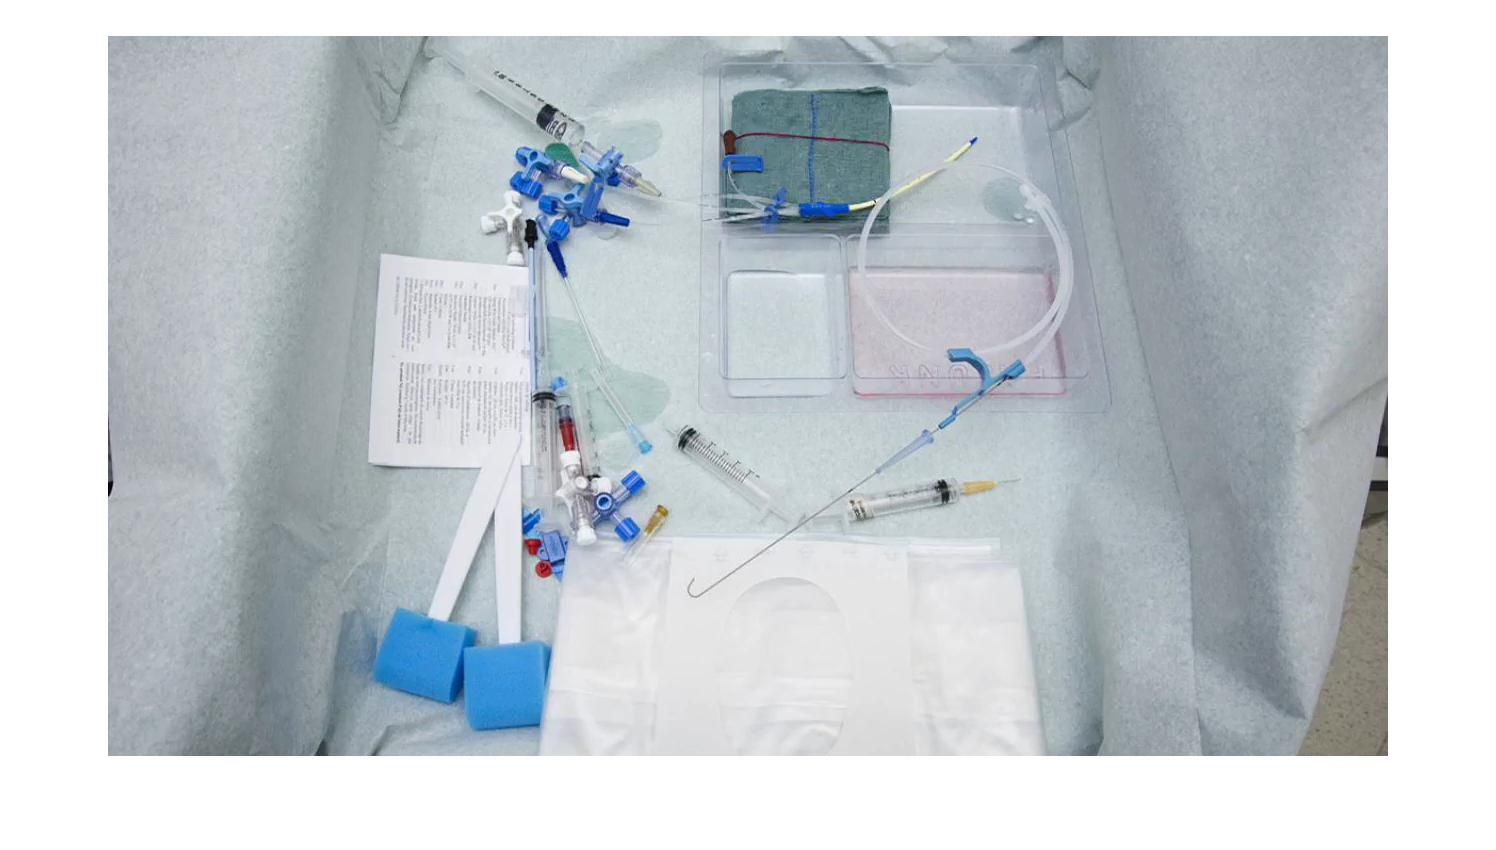
\includegraphics[width=10cm]{clip1.jpg}
				\centering
				\caption{A surgical equipment tray, with spillage under the needle}
			\end{figure}
			The data collection from the previous research project was based around a supervised eye tracking experiment in which a mixture of Expert and non-Expert Anaesthetists were asked to view a sequence of videos. These videos each depicted a scenario common to the practise, viewing an ECG screen, a surgical equipment tray etc., with a noticeable medical error in each. The subjects were prompted at the beginning of the exercise to look for these errors.
			
			During the project I carried out, I preprocessed the gaze data, filtering out variables that I felt weren't relevant to this problem, these were measurements taken by the Tobii camera and didn't serve a purpose for observing the subjects gaze.
			
	\newpage
	\chapter{Approach}
		My solution for this problem focuses on feature extraction from the Tobii gaze data files. These features are then reduced in dimensionality into a linear combination that allowed me to visualise any distinction between the two groups.
		\section{Data Visualisation}
			\subsection{Eye tracking overlay}
				\begin{figure}[h]
					\includegraphics[width=8cm]{eyeoverlay}
					\centering
					\caption{The first clip from the video, with the left (red), right (blue) and centre(black) gaze points of an expert}
				\end{figure}
				At first I decided it best to visualise the data, in the hopes that a difference in the subjects' viewing habits would be made plain. I overlaid the gaze data per frame of the eye tracking file on the corresponding frame of the video. This allowed me to follow the subjects gaze, and by comparing and contrasting subjects for different clips, I would hopefully be able to see any difference. 
				
				This view of the data was important as early on I thought to apply a Hidden Markov Model to each clip, given a model for the clip I aimed to separate any outliers, subjects who didn't behave as expected by the model, into a separate class from those who did. This did not prove viable as from the videos it was clear that while experts may spend the same time in certain areas of the screen, they did not visit each area in the same sequence, a characteristic necessary to HMMs.
			\subsection{Gaze Data Clustering}
				\begin{figure}[h]
					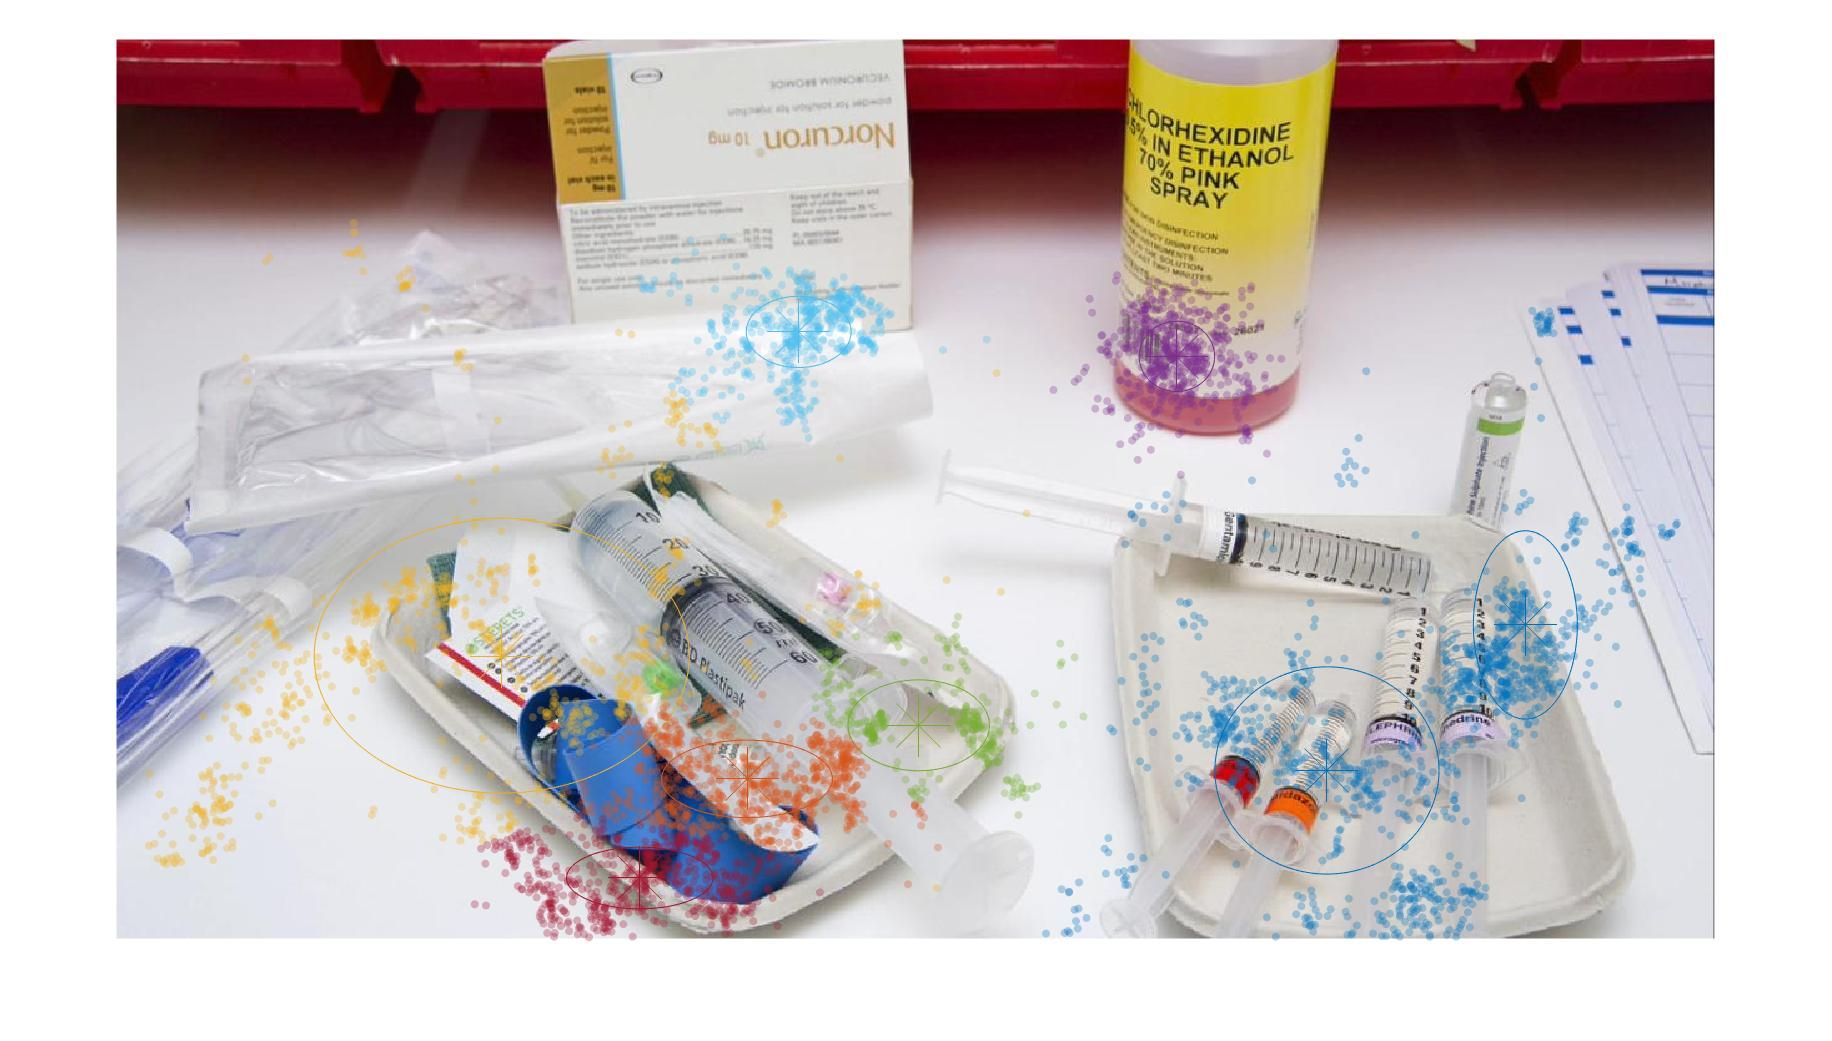
\includegraphics[width=10cm]{expertcluster}
					\centering
					\caption{Here I have clustered the eye tracking data for all experts as they viewed the 3rd clip using GMMs}
				\end{figure}
				A second approach was to cluster the gaze data of one group together over all the clip on to a freeze frame of the clip. Since the first 6 clips within the exercise video were scenes displayed in static images, the background was not temporally significant, and I could compare the subjects from the same group together in order to create a heat map of sorts. For clustering I originally used the k-means clustering algorithm, but the clusters would often overlap or envelop smaller clusters entirely. k-Means clustering works by fitting the n observations into k sets \(S = \{S_{1},S_{2}, ..., S_{k}\}\), then minimising the variance per set \footnote[1]{\texttt{https://en.wikipedia.org/wiki/K-means\_clustering}}.
				
				I account the poor clustering to the k-means algorithms unsuitability for my data, as clusters were rarely circular. I found that clustering using a Gaussian Mixture model was much more suited as, rather than a hard border being fitted to each cluster, it instead fits a gaussian blob \footnote[2]{\texttt{https://en.wikipedia.org/wiki/Mixture\_model\#Gaussian\_mixture\_model}}. The implementation first fits cluster centres using the k-Means algorithm, but then assigns data to gaussians centred around these points. By measuring the posterior probability of a gaze point belonging to each of the Gaussians in the model, I could determine that points membership to each of them. This accounts for points that are on the margin of two clusters for example.
				
				My process was then to fit a GMM to a groups data for each clip, resulting in 28 models. One requirement of clustering is to provide the number of centres to be fitted to the data. This could quite easily make the difference between good and bad clustering as assigning an incorrect number of centres could lead to two clusters being misidentified as one, or one gaussian enveloping all other data and containing any points too far from other centres to be considered as part of them, for example. However, rather than specify the number of centres based on how many clusters I could identify in each of 28 images, I implemented a heuristic using the elbow method by incrementally increasing the number of centres, measuring the percentage of variance explained and defining a cutoff point where the gradient suddenly decreases (giving the appearance of an elbow in the graph). Percentage of variance explained is defined as the ratio of between-cluster variance to overall variance.
				
				One significant drawback with this approach to the data visualisation however, was that 7 of the 14 clips were video clips, featuring temporally dynamic stimuli, in the form of waveforms on an ECG. As the point of focus would likely move with the stimuli, removing the temporal aspect from the data would result in clusters that spanned the length of the waveform section on the screen, giving little insight into focus in a spatial respect around the crest of the wave.
				\begin{figure}[h]
					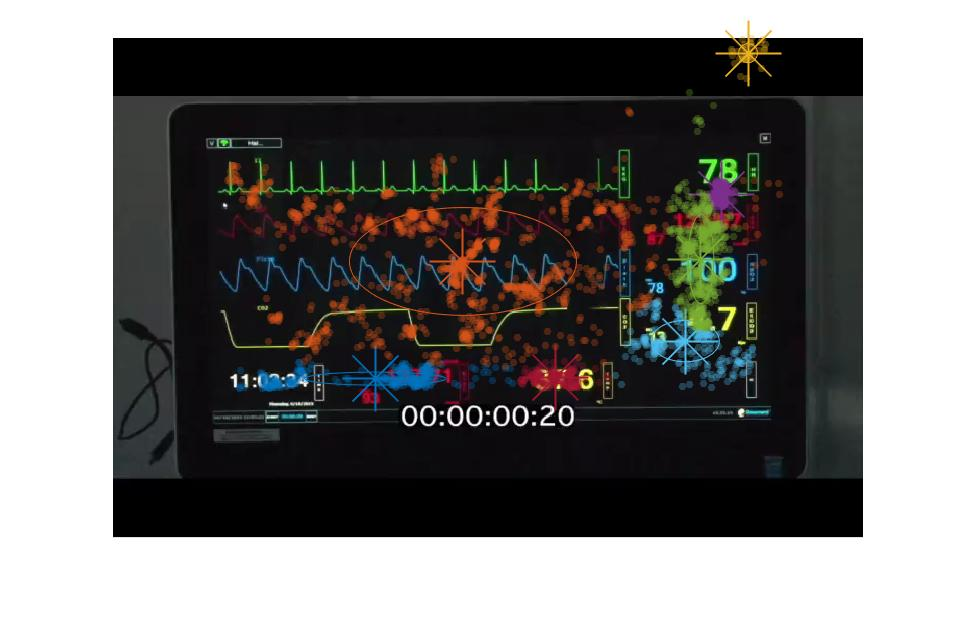
\includegraphics[width=10cm]{videocluster}
					\centering
					\caption{Poor clustering in the clip 7 due to objects moving along the screen}
				\end{figure}
				This caused feature
		\newpage
		\section{Feature Extraction}
			Classification on the raw gaze data alone is implausible. This is because both groups would visit the same areas in the image, quite possibly at the same time, as all stimuli in the image do not require any expertise to notice, rather it is in understanding them the distinction between groups would lie. Practically this means on a two dimensional space (the eye tracking data) both groups would be indiscriminable, making the task of finding a hyperplane between them (meaningless)?. However, so long as behaviour of subjects sharing a group is similar, and as a whole different from subjects in the other group, feature extraction should provide significantly separable groups of subjects, matching their class.
			
			I also decided to measure the features repeatedly throughout the clip for all subjects, splitting the clip into sections. The reasoning behind this was that while an experts activity over the whole clip might not be meaningful enough for classification, how their activity changes over the duration of the clip could prove significant. For instance, given an experts likely familiarity with the scenes displayed in the exercise, it is logical to assume that they are able to process the apparent information faster, and they might quickly scan the clip and then rest for the remainder of the clip. Settling on measuring variables once every second, for a 15 second clip, I extracted the following features.
			\subsection{Definition of a fixation}
				Many of the features defined in this project are statistics concerning the subjects behaviour while fixating. The definition of a fixation used for this purpose follows an algorithm defined in a paper on user attention \cite{overtva}:
				\begin{enumerate}
					\item{Calculate point-to-point velocity for each sample: }
					\item{Label each sample below 25$^{\circ}$/s as belonging to a potential fixation period, otherwise as to a saccade period.}
					\item{Merge consecutive potential fixation period samples into a fixation group, removing saccade samples. The length of these groups, or in other words the fixation duration, must be higher than 100ms. Under this threshold, the samples belonging to either a saccade or short fixation group, are discarded;}
					\item{Compute the spatial coordinates of each visual fixation (as the gravity centre of the coordinates of the samples in the considered group).}
				\end{enumerate}
				This algorithm was nicely translatable into my application, with a few approximations. Firstly, to measure 100ms, I calculated the framerate of the Tobii camera, and then the number of frames recorded by the camera in 100ms. I calculated the framerate, using the total number of frames of eye tracking data \(N_{F}\) for one subjects exercise, divided by the time elapsed in seconds during the exercise, \(T\).
				\[\frac{N_{F}}{T} = \frac{16073}{320.362s} \approx 50s^{-1}\]
				At 50fps, 5 frames will transpire in 100ms. I updated my algorithm to match this, i.e. a group of potential fixations must last longer than 5 frames. 
				
				The second step was to calculate movements under 25$^{\circ}$/s. My intuition was to calculate the number of pixels per degree, making it a matter of conversion. The physical size of a pixel depends on what's known as the Dots per inch, or DPI of a screen. Monitors fall into categories for DPI, which are easily available online \footnote[1]{https://snapshop.cam/dpi/}. Estimating the size of the monitor used, and my knowledge that it was standard issue IT equipment for hospital staff, I settled on 72DPI, a figure confirmed by my medical supervisor Dr. Lim. I also made approximations of the distance the viewer sat from the screen, assuming a sitting distance of 45cm, or 17.71654in. From this I calculated the distance travelled by the gaze in pixels as a result of turning the eye 25$^{\circ}$.
				\[d_{px} = \lvert{\frac{17.71654 tan(25)}{72}}\rvert \approx 170.32px\]
				Therefore, \(1^{\circ} = \frac{170.32}{25} \approx 7px\), I used this for conversion for my implementation.

				For features that used the cluster of the gaze point, I decided it was also necessary for a fixation to remain in the same cluster for it's duration.
				
			\subsection{Clustering}
				When assigning each data point to a cluster, I decided to use the expert model for each clip. The expert clustered much more nicely, and better defined the objects in the scene. This also suited a larger decision I made whilst designing the classifier \ref{classification}
				
			\subsection{Spatial features}
				Spatial features are measures of how the subject moves around the screen, for example the distance travelled in the exercise by the gaze around the screen.
				From the overlaid eye tracking clips it appeared that Experts were more steady in their gaze, and defined a smoother path, travelling back on themselves less than the Lays seemed to. Such a distinction would make itself clear in spatial measures of the gaze data. Therefore, I calculated the mean variance within a cluster for each second long section of the clip. 
				Lays on the other hand appeared to travel quite erratically from point to point, regularly flicking back to previously visited areas and apparently losing attention much more frequently. Such behaviour would manifest itself as a huge difference in distance travelled.
				
				Another hypothesis that experts might accelerate more rapidly towards each cluster, as they recognised and honed in on the stimuli at the center of that cluster was also tested.
			\newpage
			\subsection{Temporal Features}
				\subsubsection{Cluster Features}
					Following the same logic used for Spatial features, it would stand that Experts would spend less time focusing on any area as they should recognise errors quickly from experience and training. I measured this as average duration spent in one cluster. However, as some of the clusters are quite large, with some covering around 30-40\% of the screen, it is possible that the gaze could remain in one cluster for an extended period of time without fixating for the most of that time. So as an additional measure I took the average number of fixations in a cluster.
				\subsubsection{Non-Cluster Features}
					In order to account for unsuccessful clustering, as in the ECG clips, and behaviour that might not remain within a cluster, or where the cluster is not significant, I also took a selection of temporal features that do not consider the cluster data, rather just measuring the raw gaze data.
					I recorded the time taken before the sub
			Using feature extraction on the gaze data to get variables for each subject per clip, then piping this into the SVM
		how I measure the features
		classification
			Dimensionality Reduction
				PCA
				t-SNE and non-linear DR
	
\newpage
Implementation	
	Using matlab svm lib vs libSVM	
Results and Evaluation
	\label{classification}
	classification on features as a whole
	pairwise classification
	sequential feature selection
	classification after pca
	classification on interpolated pca data with tuned parameters
	
	
Conclusions + Future Work
	talk about generalisation of expert classification
	
Reflection on Learning
Glossary
Table of Abbreviations - optional
Appendices
	\begin{thebibliography}{2}
	\bibitem{eyemovements}
	Purves D, Augustine GJ, Fitzpatrick D, et al., (2001).
	\textit{Types of Eye Movements and Their Functions 2nd edition}
	Sunderland (MA): Sinauer Associates.
	\texttt{https://www.ncbi.nlm.nih.gov/books/NBK10991/}
	\bibitem{vapnik-svms}
	Cortes, C. and Vapnik, V., (1995)
	\textit{Support-vector networks}
	Machine Learning 20(3),
	Springer
	\bibitem{overtva}
	O. Le Meur, et al., (2010).
	\textit{Overt visual attention for free-viewing and quality assessment tasks Impact of the regions of interest on a video quality metric}
	Elsevier,
	\end{thebibliography}
\end{document}
